\documentclass{prova}

\usepackage{amsmath}
\usepackage{amsfonts}

\setlength{\textheight}{25cm}

\renewcommand{\sin}{\,\mbox{sen}\,}
\newcommand{\ds}{\displaystyle}

\professor{Prof.\@ Adriano Barbosa}
\disciplina{C\'alculo de V\'arias Vari\'aveis}
\avaliacao{Final}
\curso{Matem\'atica}
\data{06/03/2024}

\begin{document}
	\cabecalho{5}  % o numero 5 indica a qnt de quadros na tabela de nota

    \textbf{Todas as respostas devem ser justificadas.}

    \begin{questionario}
        \q{(2 pts) Dada $z = y + f(x^2-y^2)$, mostre que $\ds{} y\frac{\partial
            z}{\partial x} + x\frac{\partial z}{\partial y} = x$.}
        \q{(2 pts) Dados os pontos $(1,2)$, $(2,5)$, $(4,7)$ e $f(x)=ax+b$,
           encontre os valores de $a$ e $b$ tais que \[(f(1)-2)^2 + (f(2)-5)^2 +
           (f(4)-7)^2\] seja m\'{\i}nimo.}
        \q{(2 pts) Sabendo que a derivada direcional de $f$ no ponto $(3,-2,1)$ na
            dire\c{c}\~ao $(2,-1,-2)$ \'e $-3$ e que $\|\nabla f(3,-2,1)\|=3$, calcule a
            dire\c{c}\~ao de maior crescimento de $f$ no ponto $(3,-2,1)$. Quem \'e
            $\nabla f(3,-2,1)$?}

            Lembre que: $u\cdot v = \|u\| \|v\| \cos(\theta)$

        \q{(2 pts) Sendo $f$ cont\'{\i}nua, mostre que $\ds\int_0^1 \int_{x^2}^1
           \int_0^{1-y} f(t)\ dt\ dy\ dx = \frac{2}{3}\int_0^1 (1-t)^{3/2}f(t)\
           dt$.}

           Dica: mude a ordem de integra\c{c}\~ao para $dx\ dy\ dt$.
        %\q{(2 pts) Complete os limites de integra\c{c}\~ao de modo que a igualdade
        %   abaixo seja verdadeira:}
		%    \begin{equation*}
		%    	\iint_R f(x,y)\ dA = \int_0^2 \int_\square^\square f(x,y)\ dy\ dx +
		%    	\int_2^3 \int_\square^\square f(x,y)\ dy\ dx
		%    \end{equation*}
		%    onde $R$ \'e a regi\~ao da figura abaixo.
        %    \begin{figure}[h]
        %        \centering
        %        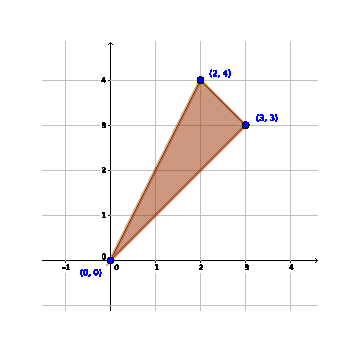
\includegraphics[width=0.4\textwidth]{fig1.pdf}
        %    \end{figure}
        \q{(2 pts) O Jacobiano de uma mudan\c{c}a de coordenadas $x=g(u,v)$ e
        $y=h(u,v)$, onde $g$ e $h$ t\^em derivadas parciais cont\'{\i}nuas, \'e dado por
        \[J=\left|\begin{array}{cc}
            \ds\frac{\partial x}{\partial u} & \ds\frac{\partial x}{\partial v} \\
            & \\
            \ds\frac{\partial y}{\partial u} & \ds\frac{\partial y}{\partial v}
        \end{array}\right|
        =\ds\frac{\partial x}{\partial u}\frac{\partial y}{\partial
        v}-\frac{\partial x}{\partial v}\frac{\partial y}{\partial u}.\]
        Podemos usar uma mudan\c{c}a de coordenadas para calcular uma integral
        dupla da seguinte forma:
        \[\iint_R f(x,y)\ dA = \iint_S f(g(u,v), h(u,v))\ |J|\ du\ dv,\]
        onde a regi\~ao $S$ do plano $uv$ \'e mapeada pela mudan\c{c}a de coordenadas
        na regi\~ao $R$ do plano $xy$.

        Use a mudan\c{c}a de coordenadas $x=\frac{1}{2}(u+v)$, $y=\frac{1}{2}(u-v)$
        para calcular a integral
        \[\iint_R e^{(x+y)/(x-y)}\ dA,\]
        onde $R$ \'e
        trap\'ezio com v\'ertices $(1,0)$, $(2,0)$, $(0,-2)$ e $(0,-1)$.} 
    \end{questionario}
\end{document}
